% ============================================================
%  Word2Vec para análisis de sentimientos en español
%  Proyecto Final - DS2011 Optimización - UTEC - Grupo 1
%
%  Compilar con:  pdflatex informe_latex.tex   (dos veces, para
%  que los números de figuras/tablas/referencias aparezcan).
%  Requiere las figuras en la carpeta results/
% ============================================================
\documentclass[11pt]{article}

\usepackage[utf8]{inputenc}
\usepackage[T1]{fontenc}
\usepackage[spanish,es-tabla]{babel}
\usepackage{amsmath,amssymb}
\usepackage{graphicx}
\usepackage{booktabs}
\usepackage{geometry}
\usepackage{float}
\usepackage{array}
\usepackage{caption}
\usepackage[hidelinks]{hyperref}

\geometry{a4paper,margin=2.5cm}
\graphicspath{{results/}}
\captionsetup{font=small,labelfont=bf}

\title{\textbf{Word2Vec para análisis de sentimientos en español:\\
arquitectura, optimización y comparación de algoritmos de entrenamiento}}
\author{Danna Nickol Gala Vásquez \and Christopher Renato Perez Torres \and
Daniel Davis Villalobos Carlos \and Paul Ricardo Maguiña Quispe \and
Oswaldo Alejandro Quispe Monzón}
\date{Curso: Optimización (DS2011) --- Docente: Victor Antonio Torrez Castillo \\ Junio 2026 --- Lima, Perú}

\begin{document}
\maketitle

% ------------------------------------------------------------
\begin{abstract}
La idea de este trabajo, en una línea, es enseñarle a una computadora a leer una reseña y
decidir si es positiva o negativa --- y mirar todo ese proceso con los lentes de la
\textbf{optimización}. Para lograrlo estudiamos \textbf{Word2Vec}, un modelo que convierte
palabras en números, y lo implementamos desde cero en PyTorch (no usamos una librería que lo
haga por nosotros). Comparamos dos arquitecturas (una y dos capas) y tres algoritmos para
entrenarlo (SGD con momentum, RMSProp y Adam), cada uno con su tasa de aprendizaje adecuada.
El estudio se arma en seis experimentos y una verificación del gradiente: comparar
arquitecturas y optimizadores; medir qué tan sensible es SGD a la tasa de aprendizaje;
rastrear la norma del gradiente para entender \emph{por qué} unos algoritmos avanzan y otros
no; comparar contra el método clásico TF-IDF; revisar la semántica que aprende el modelo;
buscar los mejores hiperparámetros; y, al final, un \emph{duelo} de nuestro modelo contra
unos embeddings preentrenados con miles de millones de palabras (SBWC), dentro y fuera de su
dominio.

Lo más importante que encontramos: (i) con su tasa adecuada, SGD sí funciona (F1-macro
$=0.861$), pero es \emph{muy} sensible a ese ajuste; a la tasa de Adam su gradiente es unas
80 veces más pequeño y se queda atascado; (ii) el mejor Word2Vec llega a F1-macro $\approx
0.89$--$0.90$; (iii) el clásico TF-IDF nos gana, incluso en su versión más simple
($0.911$), lo que dice más del problema que de nuestro modelo; (iv) la búsqueda Bayesiana no
mejora a una rejilla bien diseñada; y (v) en el duelo final, \emph{nuestro modelo le gana al
gigante preentrenado en nuestro propio dominio} ($0.903$ vs.\ $0.883$), pero el gigante
generaliza mejor fuera de él, y la razón cabe en un solo número: la cobertura de vocabulario
($82.7\%$ vs.\ $96.4\%$). Para cerrar el círculo entre teoría y práctica, verificamos
numéricamente que el gradiente que derivamos a mano es correcto.

\medskip
\noindent\textbf{Palabras clave:} Word2Vec, Skip-gram, negative sampling, descenso del
gradiente, RMSProp, Adam, Optuna, transferibilidad, NLP en español.
\end{abstract}

\tableofcontents
\newpage

% ============================================================
\section{Introducción}

\subsection{El problema, en simple}
Empecemos por el problema. Cuando alguien deja una reseña y escribe ``llegó rápido y funciona
genial'', cualquier persona entiende de inmediato que está satisfecha. Una computadora, en
cambio, solo ve una secuencia de símbolos sin significado. En el fondo, todo este proyecto
consiste en enseñarle a la máquina a dar ese salto: de letras a sentimiento.

\subsection{¿Qué tiene que ver con Optimización?}
Una relación muy directa. Cada decisión que tomamos para que el modelo aprenda se reduce a
dos cosas: definir una \textbf{función de error} ---un número que mide qué tan equivocado
está el modelo--- y buscar, paso a paso, cómo reducir ese número. Ese descenso gradual del
error es, precisamente, optimizar. Dicho de otro modo, debajo de un problema de lenguaje se
esconde un problema de optimización pura y dura, y eso es lo que iremos destapando.

Los temas del curso que aparecen explícitamente son: los \emph{métodos gradientes} (SGD como
caso base), la \emph{regresión logística} (el clasificador final y la forma de nuestra
función de pérdida), los \emph{métodos cuasi-Newton} (RMSProp y Adam, que adaptan el paso
usando información parecida a la de segundo orden) y las \emph{redes neuronales con
backpropagation} (Word2Vec es una red poco profunda). Como valor agregado, incluimos una
\emph{verificación numérica del gradiente}: derivamos la fórmula a mano y comprobamos que
está bien.

\subsection{Cómo está organizado el documento}
Seguimos el flujo natural de un experimento: primero la teoría (Sección~\ref{sec:teoria}),
luego cómo lo montamos (Sección~\ref{sec:metodo}), después qué salió (Sección~\ref{sec:resultados}),
el análisis de esos resultados (Sección~\ref{sec:analisis}) y las conclusiones
(Sección~\ref{sec:conclusiones}).

% ============================================================
\section{Planteamiento del problema}

\subsection{Pregunta de investigación}
\emph{¿Cómo afecta la elección del algoritmo de optimización (SGD, RMSProp, Adam) y la
profundidad de la red (1 vs.\ 2 capas) al entrenamiento de Word2Vec y a la calidad de los
vectores que produce? Y una vez que tenemos nuestro mejor modelo, ¿cómo se compara contra
embeddings preentrenados en un corpus gigantesco?}

\subsection{Hipótesis de trabajo}
Antes de correr nada, escribimos lo que esperábamos que pasara. Esto importa: varias de estas
hipótesis terminaron \emph{refutadas}, y reportarlo honestamente es parte del trabajo.
\begin{description}
  \item[H1.] Los métodos adaptativos (RMSProp, Adam) convergerán más rápido y a menor error
  que SGD \emph{usando la misma tasa de aprendizaje}.
  \item[H2.] La arquitectura de 2 capas producirá mejores vectores y, por tanto, mejor
  clasificación que la de 1 capa.
  \item[H3.] SGD es más sensible a la tasa de aprendizaje que Adam: solo funciona en un rango
  estrecho, mientras Adam aguanta variaciones de varios órdenes de magnitud.
  \item[H4.] Word2Vec superará a TF-IDF porque captura relaciones de significado que el
  método clásico no puede ver.
  \item[H5.] La búsqueda Bayesiana (Optuna) encontrará una configuración bastante mejor que
  una búsqueda en rejilla.
  \item[H6.] Los embeddings preentrenados en un corpus enorme (SBWC) generalizarán mejor
  \emph{fuera de dominio} que los nuestros, entrenados con apenas 40\,000 reseñas.
\end{description}

% ============================================================
\section{Marco teórico}\label{sec:teoria}

\subsection{Del texto a los vectores: el problema de fondo}
La forma más simple de darle texto a una computadora es la \emph{bag-of-words}: un vector
gigante donde cada posición cuenta cuántas veces aparece una palabra. Tiene dos problemas. El
primero es de tamaño: con decenas de miles de palabras, esos vectores son enormes y casi
todos ceros. El segundo es más sutil pero más grave: no hay noción de significado. Para ese
método, ``bueno'' y ``excelente'' son tan distintos entre sí como ``bueno'' y ``mesa'', porque
cada palabra vive en su propia posición sin relación con las demás. Word2Vec ataca justamente
esos dos problemas.

\subsection{La idea central de Word2Vec}
Antes de la fórmula, la idea en simple. Para que la máquina trabaje con palabras, primero hay
que convertirlas en números. Word2Vec lo hace con una idea elegante: ubica cada palabra como
un punto en un espacio, de modo que las palabras de significado parecido queden cerca y las
distintas, lejos. Es como un mapa, pero de palabras en lugar de ciudades: ``excelente'' y
``perfecto'' quedarían en la misma vecindad; ``excelente'' y ``horrible'', en extremos
opuestos.

¿Y cómo decide la máquina quién está cerca de quién, si nadie le explicó el significado de
cada palabra? A partir del contexto: si dos palabras suelen aparecer rodeadas de las mismas
palabras, es muy probable que signifiquen algo parecido. Esta intuición tiene nombre propio
---la \textbf{hipótesis distribucional}~\cite{harris1954}--- y es el corazón de Word2Vec~\cite{mikolov2013a}.

\subsection{Arquitectura Skip-gram}
Word2Vec tiene dos sabores; nosotros usamos \textbf{Skip-gram}, que funciona así: toma una
palabra y trata de adivinar qué palabras la rodean. Entrenando millones de veces esa tarea
de ``adivina el vecindario'', los vectores se acomodan solos para que las palabras que
comparten contexto queden cercanas. Formalmente, para un corpus $w_1,\dots,w_T$ y una ventana
de tamaño $c$, busca maximizar la probabilidad de los vecinos:
\begin{equation}
\mathcal{L}_{SG} = \frac{1}{T}\sum_{t=1}^{T}\sum_{-c\le j\le c,\, j\ne 0}
\log P(w_{t+j}\mid w_t).
\end{equation}
Esa probabilidad se calcula, en teoría, con un \emph{softmax} que compara la palabra contra
\emph{todo} el vocabulario. El problema: con miles de palabras, hacer esa cuenta en cada paso
es carísimo. La solución se llama \emph{negative sampling}.

\subsection{Negative Sampling: nuestra función de pérdida}
La intuición del truco es bonita. En vez de preguntarle al modelo ``¿cuál de las 9\,597
palabras del vocabulario es el vecino correcto?'' (carísimo), le hacemos una pregunta mucho
más barata: ``aquí tienes el vecino verdadero y unas pocas palabras al azar; ¿sabes
distinguir al verdadero de los impostores?''. Eso convierte el problema en una simple
clasificación binaria. Para un par positivo $(w_I, w_O)$ con $K$ negativos $\{w_k\}$, la
pérdida es~\cite{mikolov2013b}:
\begin{equation}\label{eq:ns}
\mathcal{L}_{NS} = -\log\sigma\!\left(\mathbf{v}_{w_O}^{\top}\mathbf{u}_{w_I}\right)
- \sum_{k=1}^{K}\log\sigma\!\left(-\mathbf{v}_{w_k}^{\top}\mathbf{u}_{w_I}\right),
\end{equation}
donde $\sigma(x)=1/(1+e^{-x})$ es la sigmoide y los negativos se sacan de una distribución
$P_n(w)\propto f(w)^{3/4}$. Detalle que conecta con el curso: la Ecuación~\eqref{eq:ns} es
exactamente una \textbf{entropía cruzada binaria}, la misma de la regresión logística.
Minimizarla respecto a los vectores $\mathbf{u}$ y $\mathbf{v}$ es el problema de
optimización que resolvemos.

\subsection{El gradiente: hacia dónde empujar}
Para minimizar la pérdida necesitamos su gradiente, que nos dice en qué dirección mover cada
vector. El del vector de entrada $\mathbf{u}_{w_I}$ es:
\begin{equation}\label{eq:grad}
\frac{\partial \mathcal{L}_{NS}}{\partial \mathbf{u}_{w_I}} =
\left[\sigma\!\left(\mathbf{v}_{w_O}^{\top}\mathbf{u}_{w_I}\right)-1\right]\mathbf{v}_{w_O}
+ \sum_{k=1}^{K}\sigma\!\left(\mathbf{v}_{w_k}^{\top}\mathbf{u}_{w_I}\right)\mathbf{v}_{w_k}.
\end{equation}
Leída en palabras, esta fórmula hace algo muy intuitivo: \emph{acerca} la palabra central a
su contexto real y la \emph{aleja} de las palabras al azar. Repetido millones de veces, ese
empujón es el que va formando el ``mapa de palabras''. Más adelante (Sección~\ref{sec:gradcheck})
comprobamos numéricamente que esta fórmula está bien derivada.

\subsection{Un punto fino: este problema NO es convexo}\label{sec:convexidad}
Vale la pena aclarar algo que suele malinterpretarse. Un problema convexo es como un tazón:
tiene un único fondo y siempre llegas a él. Uno no convexo es como una cordillera llena de
valles: dependiendo de por dónde bajes, puedes quedar atrapado en un valle que no es el más
profundo. \textbf{Nuestra pérdida es no convexa, incluso con una sola capa.} La razón es que
en $\sigma(\mathbf{v}^{\top}\mathbf{u})$ aparecen multiplicados los dos vectores que estamos
ajustando, y esa multiplicación entre incógnitas (bilinealidad) crea ese paisaje accidentado.
La extensión a dos capas con $\tanh$ \emph{agrega} más relieve, pero el terreno ya era
irregular de origen. Esto es justo lo que hace interesante comparar optimizadores: el
resultado depende de cómo cada algoritmo navega esa cordillera.

\subsection{La extensión de dos capas}
Probamos también una versión con una capa extra, que mete una transformación no lineal entre
el vector de entrada y la comparación final:
\begin{align}
\mathbf{h} &= \tanh(W_2\,\mathbf{u}_{w_I}+\mathbf{b})\in\mathbb{R}^{d_h},\\
\mathcal{L}_{2L} &= -\log\sigma\!\left(\mathbf{v}_{w_O}^{\top}\mathbf{h}\right)
- \sum_{k=1}^{K}\log\sigma\!\left(-\mathbf{v}_{w_k}^{\top}\mathbf{h}\right).
\end{align}
La idea era que esa capa extra aprendiera representaciones más ricas. Si funcionó o no, lo
vemos en los resultados.

\subsection{Los tres optimizadores}
Aquí está el corazón del curso. Entrenar es como bajar una montaña con niebla: no ves el
fondo, solo sientes la pendiente bajo tus pies (el gradiente) y decides hacia dónde dar el
siguiente paso. Lo que cambia entre algoritmos es \emph{cómo} eligen ese paso.

\paragraph{SGD con momentum.} El descenso del gradiente estocástico da un paso en contra de la
pendiente. Le agregamos \emph{momentum}: como una pelota que rueda cuesta abajo, acumula
inercia y no se detiene ante cada pequeña irregularidad.
\begin{equation}\label{eq:sgd}
\mathbf{m}_{t+1}=\mu\,\mathbf{m}_t+\nabla_\theta \mathcal{L}(\theta_t),\qquad
\theta_{t+1}=\theta_t-\eta\,\mathbf{m}_{t+1},\qquad \mu=0.9.
\end{equation}
El momentum no es un lujo aquí: como la matriz de salida arranca en ceros, el primer
gradiente es diminuto; sin esa inercia acumulada, SGD ni siquiera se mueve del punto de
partida. Su gran debilidad es el tamaño del paso $\eta$ (la \emph{tasa de aprendizaje}): muy
grande y se pasa de largo; muy pequeño y tarda una eternidad.

\paragraph{RMSProp.} Su idea: usar un paso distinto para cada dirección, según qué tan
empinada ha venido siendo. Donde el terreno cambia brusco, pasos cortos; donde es suave,
pasos largos.
\begin{equation}
v_t=\alpha\,v_{t-1}+(1-\alpha)g_t^2,\qquad
\theta_{t+1}=\theta_t-\frac{\eta}{\sqrt{v_t}+\epsilon}\,g_t,\qquad \alpha=0.99.
\end{equation}

\paragraph{Adam.} Combina lo mejor de ambos: la inercia del momentum y el paso adaptativo de
RMSProp, con una corrección al inicio para no arrancar sesgado.
\begin{align}
m_t&=\beta_1 m_{t-1}+(1-\beta_1)g_t, & v_t&=\beta_2 v_{t-1}+(1-\beta_2)g_t^2,\\
\hat{m}_t&=\tfrac{m_t}{1-\beta_1^t}, & \hat{v}_t&=\tfrac{v_t}{1-\beta_2^t},\qquad
\theta_{t+1}=\theta_t-\frac{\eta}{\sqrt{\hat{v}_t}+\epsilon}\,\hat{m}_t,
\end{align}
con $\beta_1=0.9$ y $\beta_2=0.999$. Por eso a Adam se le suele llamar ``el optimizador que
casi siempre funciona sin que lo toques''.

\subsection{Del vector de palabra al clasificador}
Word2Vec nos da un vector por palabra, pero una reseña tiene muchas palabras. La receta
simple: el vector de un documento es el \emph{promedio} de los vectores de sus palabras,
$\mathbf{d}=\frac{1}{|T_{doc}|}\sum_{w}\mathbf{u}_w$. Sobre ese promedio entrenamos una
\textbf{Regresión Logística} que decide positivo o negativo. (Promediar tiene un costo: se
pierde el orden de las palabras, algo que retomamos en las limitaciones.)

% ============================================================
\section{Metodología}\label{sec:metodo}

\subsection{El dataset}
Usamos \texttt{amazon\_reviews\_multi}~\cite{keung2020} en español (vía MTEB~\cite{muennighoff2023}):
reseñas con calificación de 1 a 5 estrellas. Lo volvimos un problema binario: 1--2 estrellas
es negativo, 4--5 es positivo, y las de 3 (ambiguas) las descartamos. Entrenamos sobre un
subconjunto balanceado de 40\,000 reseñas (Cuadro~\ref{tab:dataset}). Elegimos este corpus
porque es grande, está escrito en español nativo y las estrellas son una etiqueta de
sentimiento confiable (las pone el propio comprador).
\begin{table}[H]
\centering
\caption{Particiones del dataset tras volverlo binario.}\label{tab:dataset}
\begin{tabular}{lccc}
\toprule
Partición & Total & Negativo & Positivo \\
\midrule
Entrenamiento & 40\,000 & 19\,838 & 20\,162 \\
Validación & 4\,000 & $\approx$2\,000 & $\approx$2\,000 \\
Test & 4\,000 & $\approx$2\,000 & $\approx$2\,000 \\
\bottomrule
\end{tabular}
\end{table}

\subsection{Preprocesamiento}
Lo dejamos a propósito mínimo, para no borrar señal útil: pasar a minúsculas, quitar URLs y
menciones, eliminar puntuación y dígitos, separar por espacios y descartar tokens de una sola
letra. Con \texttt{min\_count}=5 (ignorar palabras que aparecen menos de 5 veces), el
vocabulario quedó en \textbf{9\,597 palabras}.

\subsection{Configuración y una decisión importante}
El Cuadro~\ref{tab:hparams} lista los hiperparámetros base. La lógica: fijamos $d=100$ y todo
lo demás para comparar limpio el efecto del optimizador y la arquitectura; después
exploramos la dimensión y la tasa por separado. Todas las corridas fijan una semilla aleatoria
($=42$) para que los resultados sean reproducibles.
\begin{table}[H]
\centering
\caption{Hiperparámetros base del experimento principal.}\label{tab:hparams}
\begin{tabular}{lcl}
\toprule
Hiperparámetro & Valor & Qué es \\
\midrule
Dimensión de embeddings $d$ & 100 & Tamaño del vector de cada palabra (control fijo) \\
Dimensión capa oculta $d_h$ & 64 & Solo en la versión de 2 capas \\
Ventana de contexto $c$ & 5 & Cuántas palabras a cada lado se consideran vecinas \\
Negativos por par $K$ & 5 & Cuántos ``impostores'' por cada vecino real \\
Épocas & 5 & Pasadas completas por el corpus (7 en exp1/exp2) \\
Tamaño de batch & 512 & Pares por actualización \\
\bottomrule
\end{tabular}
\end{table}

\paragraph{Una tasa de aprendizaje por optimizador.} Esto nos lo cuestionamos bastante.
Comparar los tres optimizadores con la \emph{misma} tasa parece justo, pero no lo es: $0.001$
es la tasa cómoda de Adam y RMSProp, pero a SGD lo deja paralizado. Sería como hacer correr
los 100 metros a tres atletas con la misma talla de zapatillas. Así que le dimos a cada uno
su tasa adecuada: \textbf{SGD con $\eta=0.1$}, \textbf{RMSProp y Adam con $\eta=0.001$}. La
sensibilidad de SGD a ese ajuste la estudiamos aparte (exp1), que es donde realmente brilla
esa observación.

% ============================================================
\section{Resultados}\label{sec:resultados}

\subsection{Curvas de convergencia: ¿bajan el error?}
Lo primero es mirar si el entrenamiento de verdad reduce la pérdida época tras época
(Figuras~\ref{fig:conv1} y~\ref{fig:conv2}). Con su tasa adecuada, los tres optimizadores
bajan; SGD parte más arriba y desciende más lento que los adaptativos, pero ya no se queda
clavado como veremos que pasa cuando le ponemos una tasa equivocada.
\begin{figure}[H]
\centering
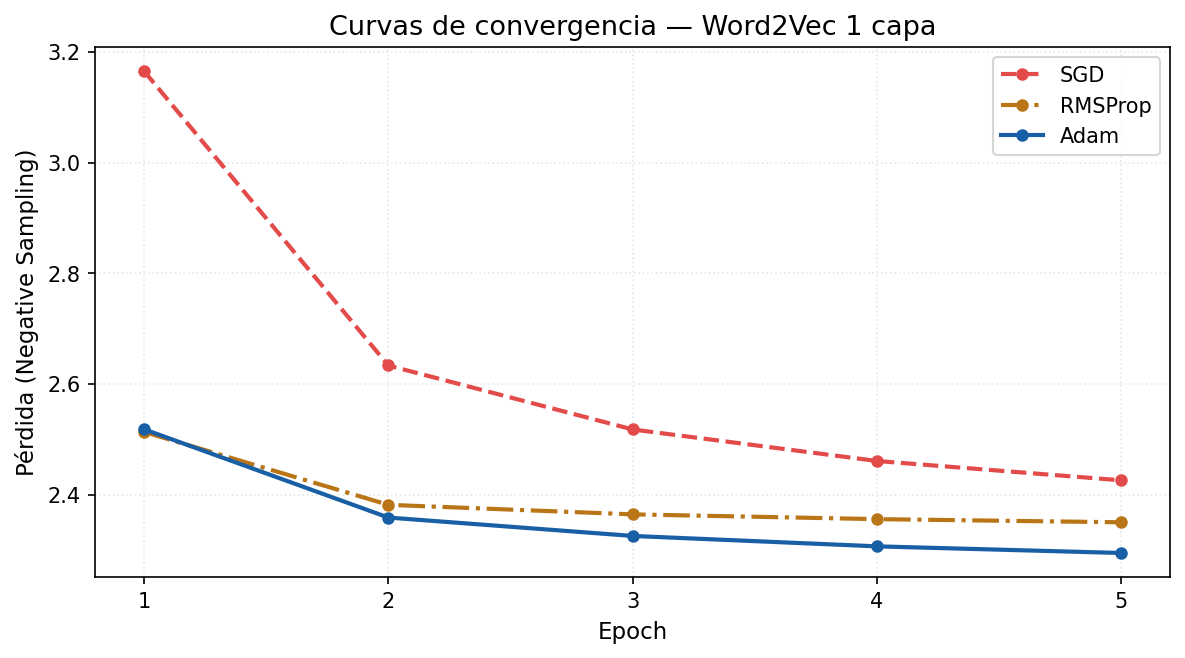
\includegraphics[width=0.72\textwidth]{convergencia_1_capa.png}
\caption{Curvas de convergencia --- Word2Vec de 1 capa.}\label{fig:conv1}
\end{figure}
\begin{figure}[H]
\centering
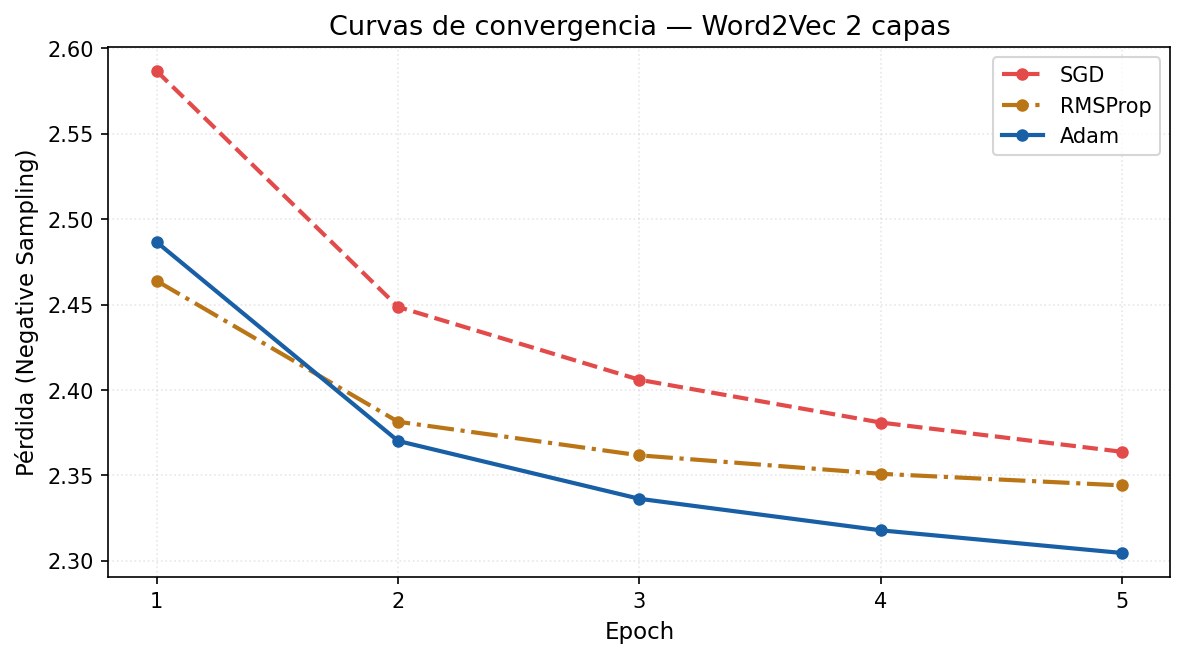
\includegraphics[width=0.72\textwidth]{convergencia_2_capas.png}
\caption{Curvas de convergencia --- Word2Vec de 2 capas.}\label{fig:conv2}
\end{figure}

\subsection{Resultados de clasificación}
El Cuadro~\ref{tab:main} es el resultado central: qué tan bien clasifica cada combinación,
medido con F1-macro (un promedio justo entre acertar positivos y negativos). El ganador es
1 capa con RMSProp.
\begin{table}[H]
\centering
\caption{Clasificación en test (4\,000 reseñas). Cada optimizador con su $\eta$ adecuada.}
\label{tab:main}
\begin{tabular}{llcccc}
\toprule
Arquitectura & Optimizador & $\eta$ & Accuracy & F1-macro & Tiempo (s) \\
\midrule
1 capa  & SGD     & 0.1   & 0.8608 & 0.8607 & 221 \\
1 capa  & RMSProp & 0.001 & 0.8940 & \textbf{0.8940} & 183 \\
1 capa  & Adam    & 0.001 & 0.8932 & 0.8932 & 188 \\
2 capas & SGD     & 0.1   & 0.8812 & 0.8812 & 302 \\
2 capas & RMSProp & 0.001 & 0.8822 & 0.8822 & 181 \\
2 capas & Adam    & 0.001 & 0.8900 & 0.8900 & 198 \\
\bottomrule
\end{tabular}
\end{table}
\noindent\textbf{Qué significa.} Tres lecturas rápidas: los métodos adaptativos (RMSProp,
Adam) van un pelo por delante; la segunda capa \emph{no} ayuda (las de 2 capas no superan a
la mejor de 1 capa); y SGD, con su tasa, queda competitivo aunque no gana.

\subsection{Visualización: ¿el mapa de palabras existe?}
Para ver si Word2Vec de verdad aprendió un ``mapa de palabras'', usamos t-SNE (una técnica que
aplana un espacio de muchas dimensiones a un plano de 2, como aplanar un globo terráqueo en un
mapa). En la Figura~\ref{fig:tsne}, palabras relacionadas caen juntas: señal de que el modelo
capturó estructura semántica.
\begin{figure}[H]
\centering
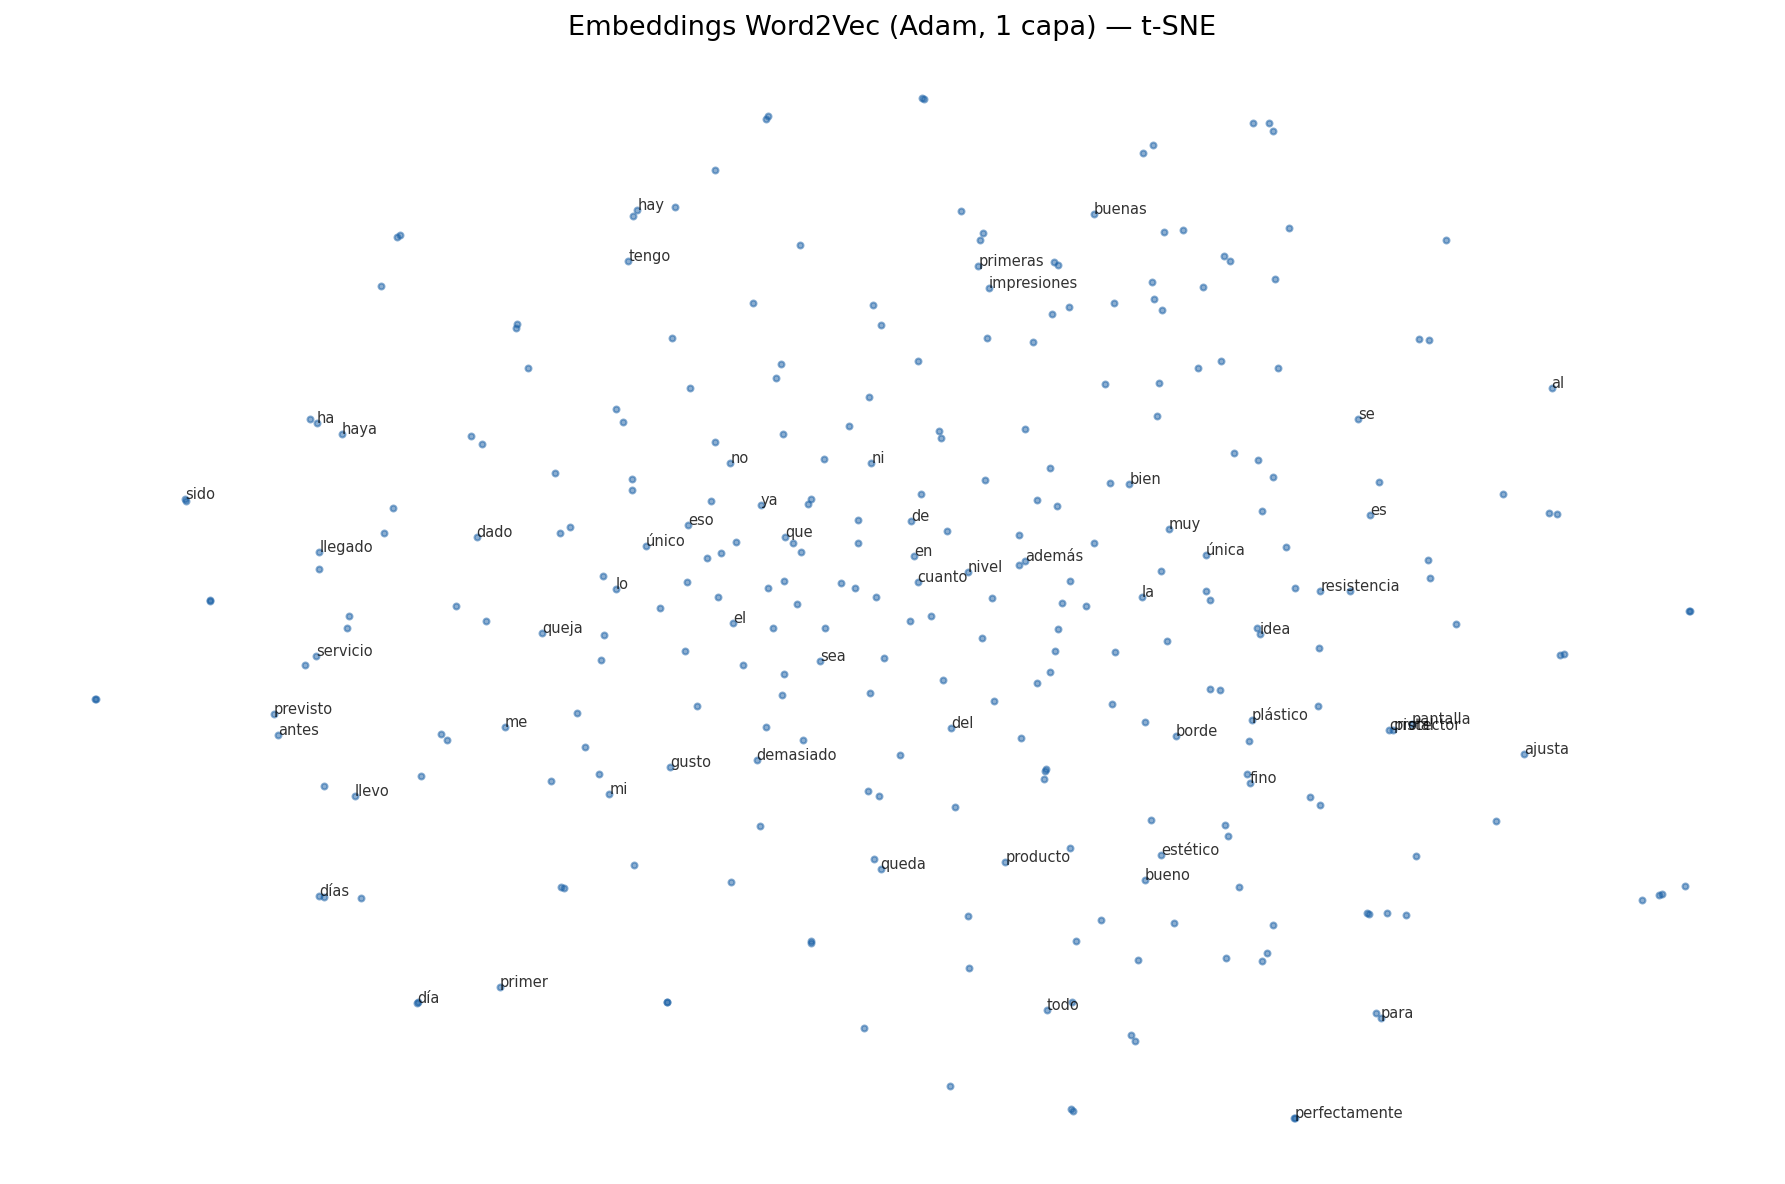
\includegraphics[width=0.68\textwidth]{tsne_embeddings.png}
\caption{Proyección t-SNE de los embeddings (1 capa, Adam).}\label{fig:tsne}
\end{figure}

\subsection{Experimento 1: ¿qué tan quisquilloso es SGD con la tasa?}
Aquí está la observación que más le gusta al curso. Tomamos el \emph{mismo} algoritmo (SGD) y
solo le cambiamos la tasa de aprendizaje. El resultado (Cuadro~\ref{tab:exp1}) es dramático:
el mismo método pasa de un F1 de $0.87$ a uno de $0.62$ según el tamaño del paso. No es que
SGD sea bueno o malo: es que es \emph{exigente} con su ajuste.
\begin{figure}[H]
\centering
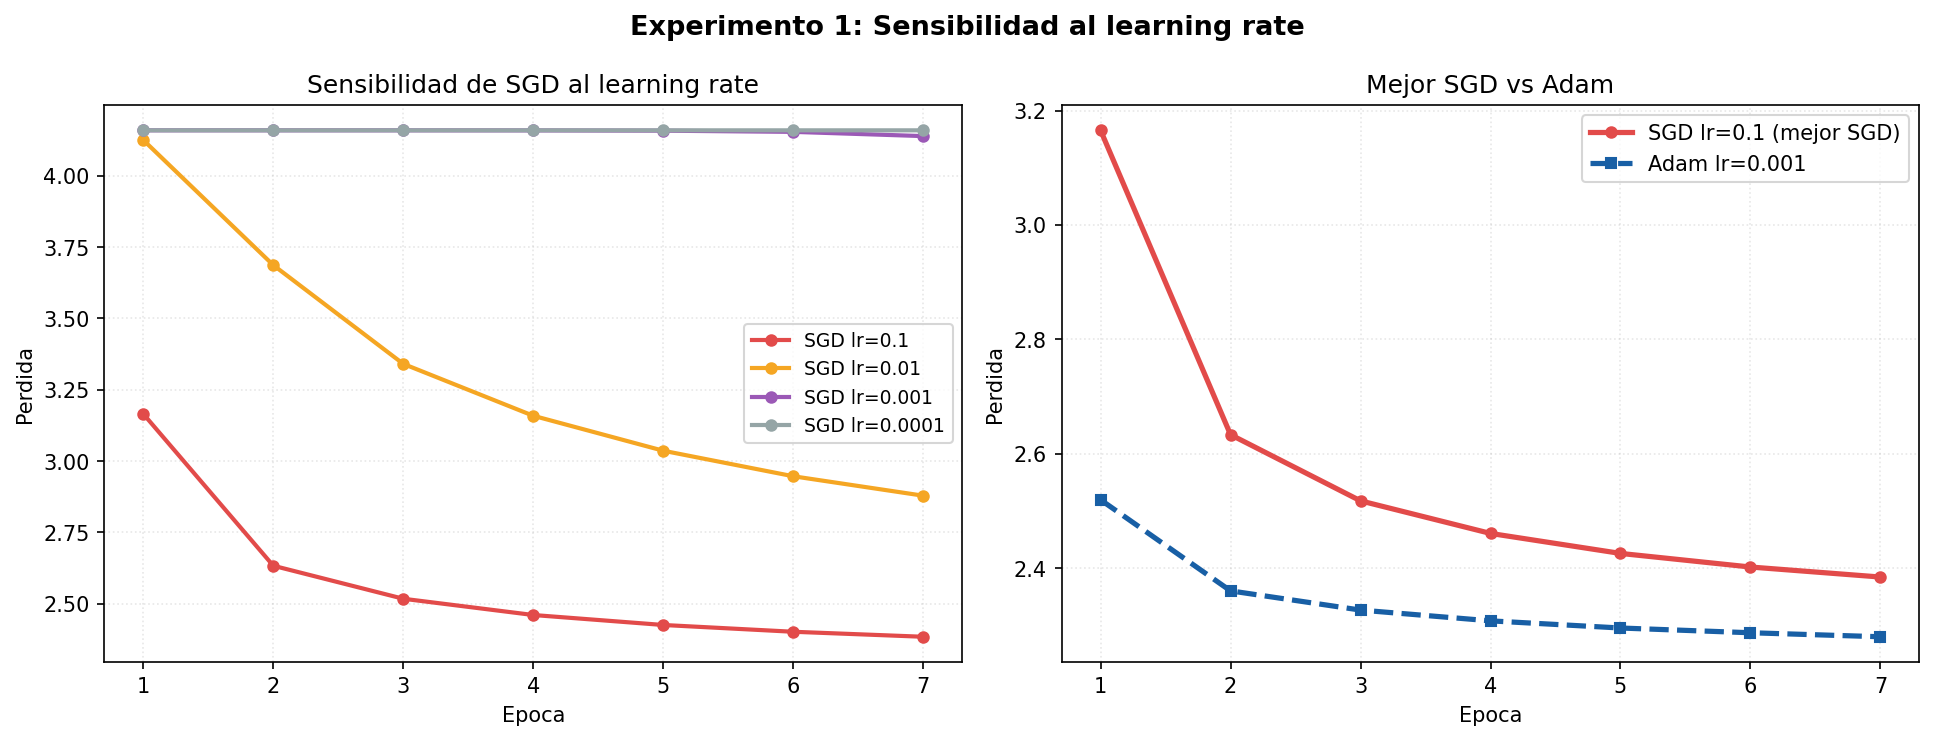
\includegraphics[width=0.85\textwidth]{exp1_lr_sensitivity.png}
\caption{Izq.: pérdida de SGD para cuatro tasas. Der.: el mejor SGD ($\eta=0.1$) frente a Adam.}
\label{fig:exp1}
\end{figure}
\begin{table}[H]
\centering
\caption{SGD según su tasa de aprendizaje (1 capa, 7 épocas).}\label{tab:exp1}
\begin{tabular}{lccl}
\toprule
Tasa $\eta$ & F1-macro & Pérdida final & Qué pasó \\
\midrule
$0.1$    & \textbf{0.8742} & 2.384 & Converge bien \\
$0.01$   & 0.7715 & 2.879 & Converge lento \\
$0.001$  & 0.6212 & 4.139 & Se queda atascado \\
$0.0001$ & 0.6829 & 4.159 & Congelado \\
\bottomrule
\end{tabular}
\end{table}

\subsection{Experimento 2: ¿por qué Adam avanza y SGD no?}
La tabla anterior muestra \emph{que} SGD se atasca a tasas pequeñas; este experimento muestra
\emph{por qué}. La idea: a igualdad de condiciones ($\eta=0.001$ para ambos), medimos la norma
del gradiente ---qué tan ``empinado'' siente el terreno cada uno--- época por época
(Figura~\ref{fig:exp2}). El gradiente de SGD es unas \textbf{80 veces más pequeño} que el de
Adam al inicio (luego la brecha baja a $\sim$7 veces). La explicación cae de madura: Adam
\emph{normaliza} el paso por el historial, así que da zancadas útiles donde SGD da pasos
ridículamente pequeños y se queda en la meseta del arranque.
\begin{figure}[H]
\centering
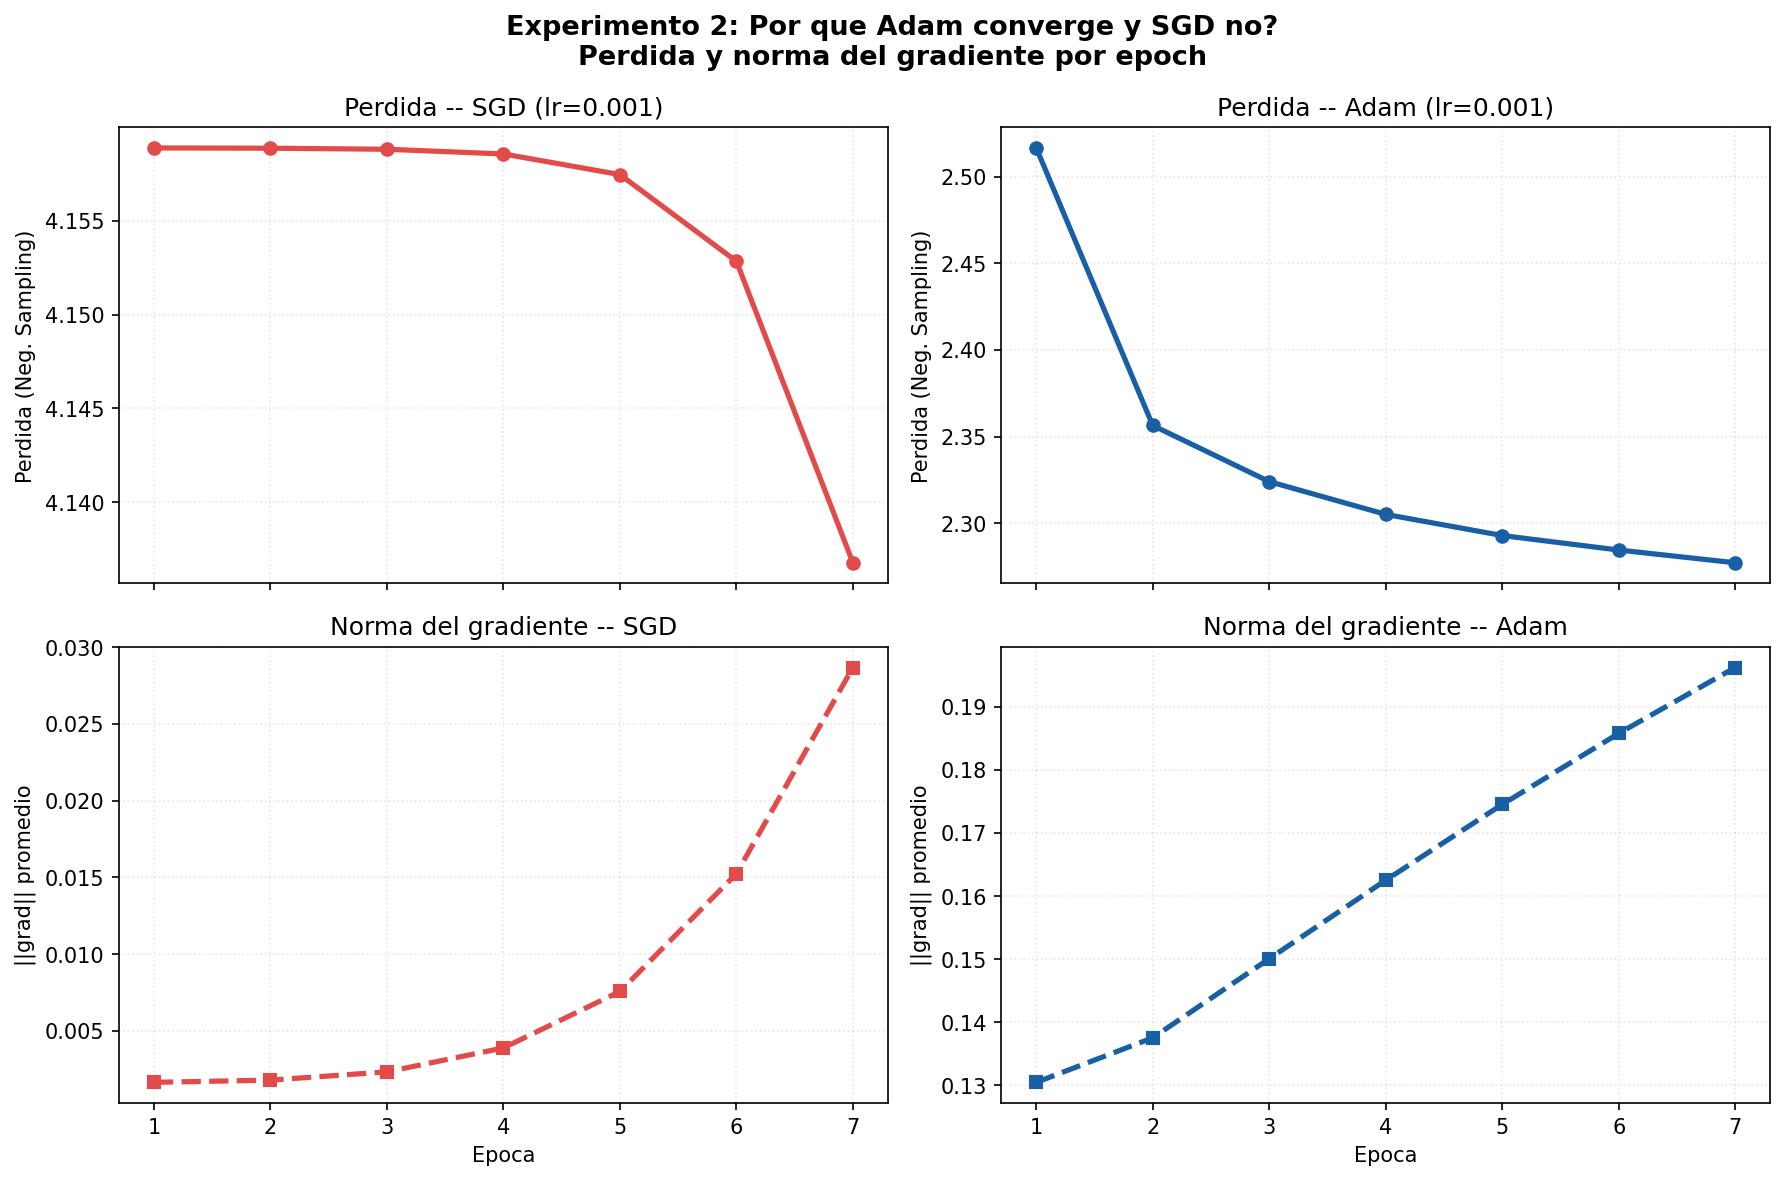
\includegraphics[width=0.85\textwidth]{exp2_grad_tracking.png}
\caption{Pérdida y norma del gradiente para SGD y Adam, ambos con $\eta=0.001$.}\label{fig:exp2}
\end{figure}

\subsection{Experimento 3: el clásico TF-IDF entra al ring}
TF-IDF es el método de la vieja escuela: básicamente cuenta qué palabras aparecen y qué tan
distintivas son, sin entender nada de significado. Lo pusimos como rival. El resultado
(Cuadro~\ref{tab:exp3}) nos sorprendió: TF-IDF gana, y lo hace \emph{incluso en su versión más
simple} (solo palabras sueltas, $0.9107$), no solo con la versión más completa de pares de
palabras ($0.9225$).
\begin{figure}[H]
\centering
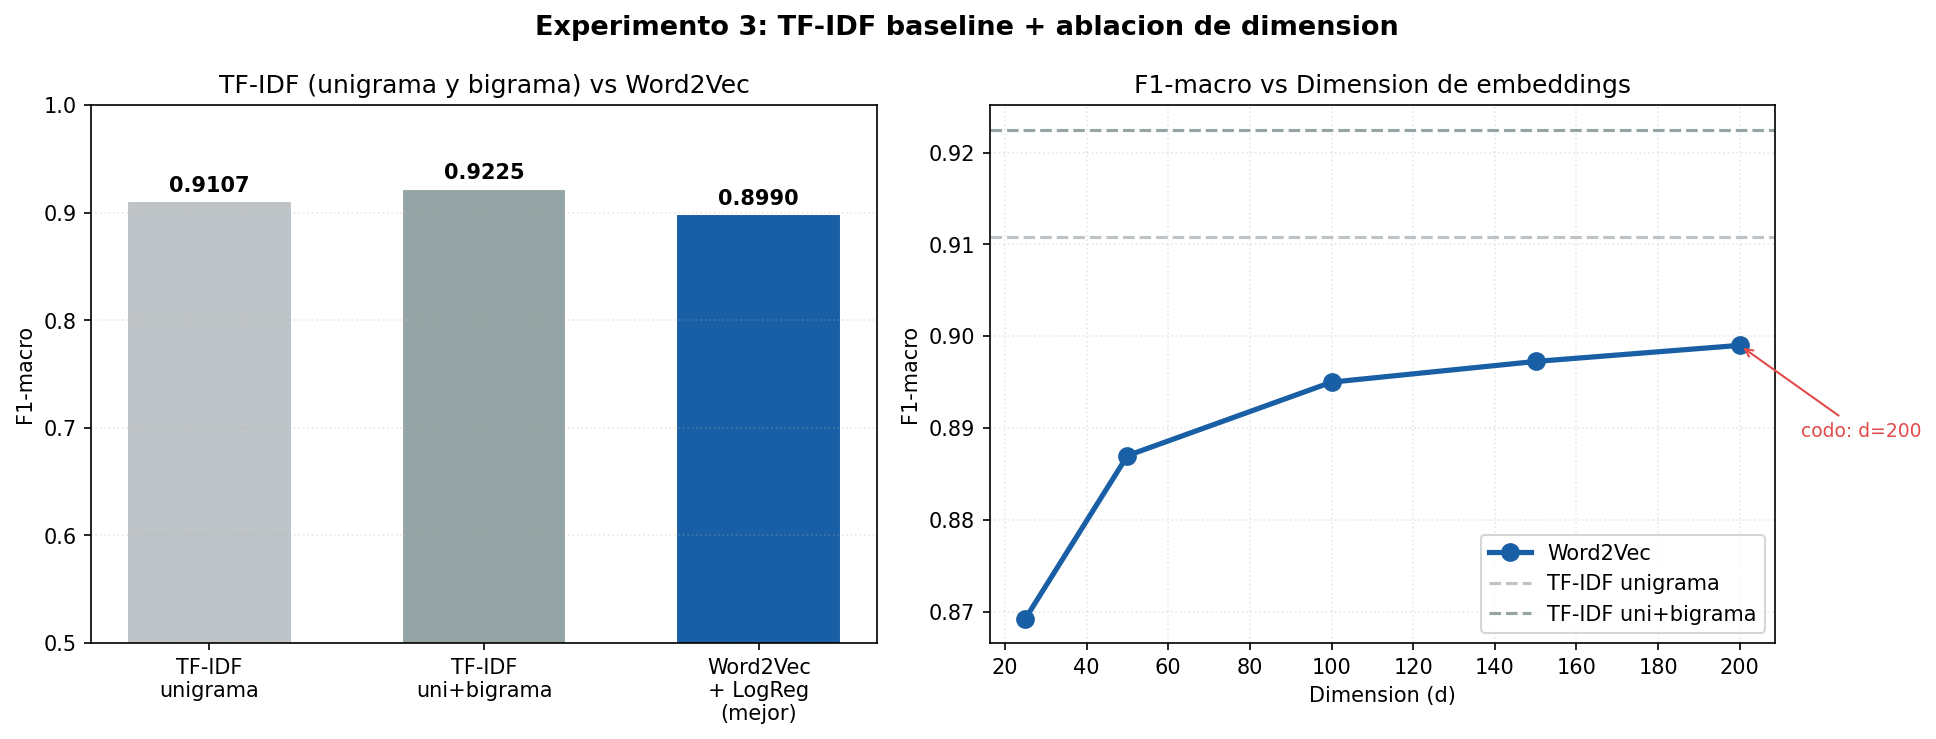
\includegraphics[width=0.85\textwidth]{exp3_tfidf_ablacion.png}
\caption{Izq.: TF-IDF (simple y con pares) vs.\ Word2Vec. Der.: F1 según la dimensión $d$.}
\label{fig:exp3}
\end{figure}
\begin{table}[H]
\centering
\caption{Dimensión de los embeddings (Adam) y el baseline TF-IDF.}\label{tab:exp3}
\begin{tabular}{lc}
\toprule
Representación & F1-macro \\
\midrule
Word2Vec $d=25$  & 0.8692 \\
Word2Vec $d=50$  & 0.8870 \\
Word2Vec $d=100$ & 0.8950 \\
Word2Vec $d=150$ & 0.8972 \\
Word2Vec $d=200$ & 0.8990 \\
\midrule
TF-IDF palabras sueltas & 0.9107 \\
TF-IDF con pares de palabras & \textbf{0.9225} \\
\bottomrule
\end{tabular}
\end{table}
\noindent\textbf{Qué significa.} Esto dice más del problema que de nuestro modelo. En las
reseñas de Amazon la gente es directísima: ``pésimo'', ``no funciona'', ``excelente''. Cuando
la sola presencia de esas palabras ya delata el sentimiento, contarlas alcanza y sobra ---
trajimos un bisturí a una tarea que se resolvía con un martillo. Word2Vec rinde cuando el
contexto importa más que la palabra suelta (ironía, dobles sentidos), algo que confirmaremos
en el duelo final.

\subsection{Experimento 4: ¿el modelo entendió de verdad?}
Una cosa es clasificar bien y otra es que los vectores tengan sentido. Para verificarlo, le
preguntamos al modelo cuáles son las palabras más parecidas a otras (Cuadro~\ref{tab:exp4}).
Las respuestas son coherentes ---incluye sinónimos y hasta faltas de ortografía del propio
corpus---, lo que muestra que los vectores son interpretables, no una caja negra.
\begin{table}[H]
\centering
\caption{Las 5 palabras más parecidas, por similitud coseno (Adam, $d=100$).}\label{tab:exp4}
\begin{tabular}{ll}
\toprule
Palabra & Vecinos más cercanos (similitud) \\
\midrule
excelente  & inmejorable (0.79), exelente (0.76), buenisimo (0.75), excepcional (0.74) \\
horrible   & fatal (0.72), pésimo (0.66), malísimo (0.62), desastre (0.57) \\
roto       & doblado (0.76), rajado (0.75), estropeado (0.73), destrozado (0.72) \\
recomiendo & aconsejo (0.77), recomendaría (0.70), recomendaria (0.69), volvería (0.64) \\
envio      & envío (0.84), envió (0.80), entrega (0.70), estimado (0.69) \\
\bottomrule
\end{tabular}
\end{table}
\begin{figure}[H]
\centering
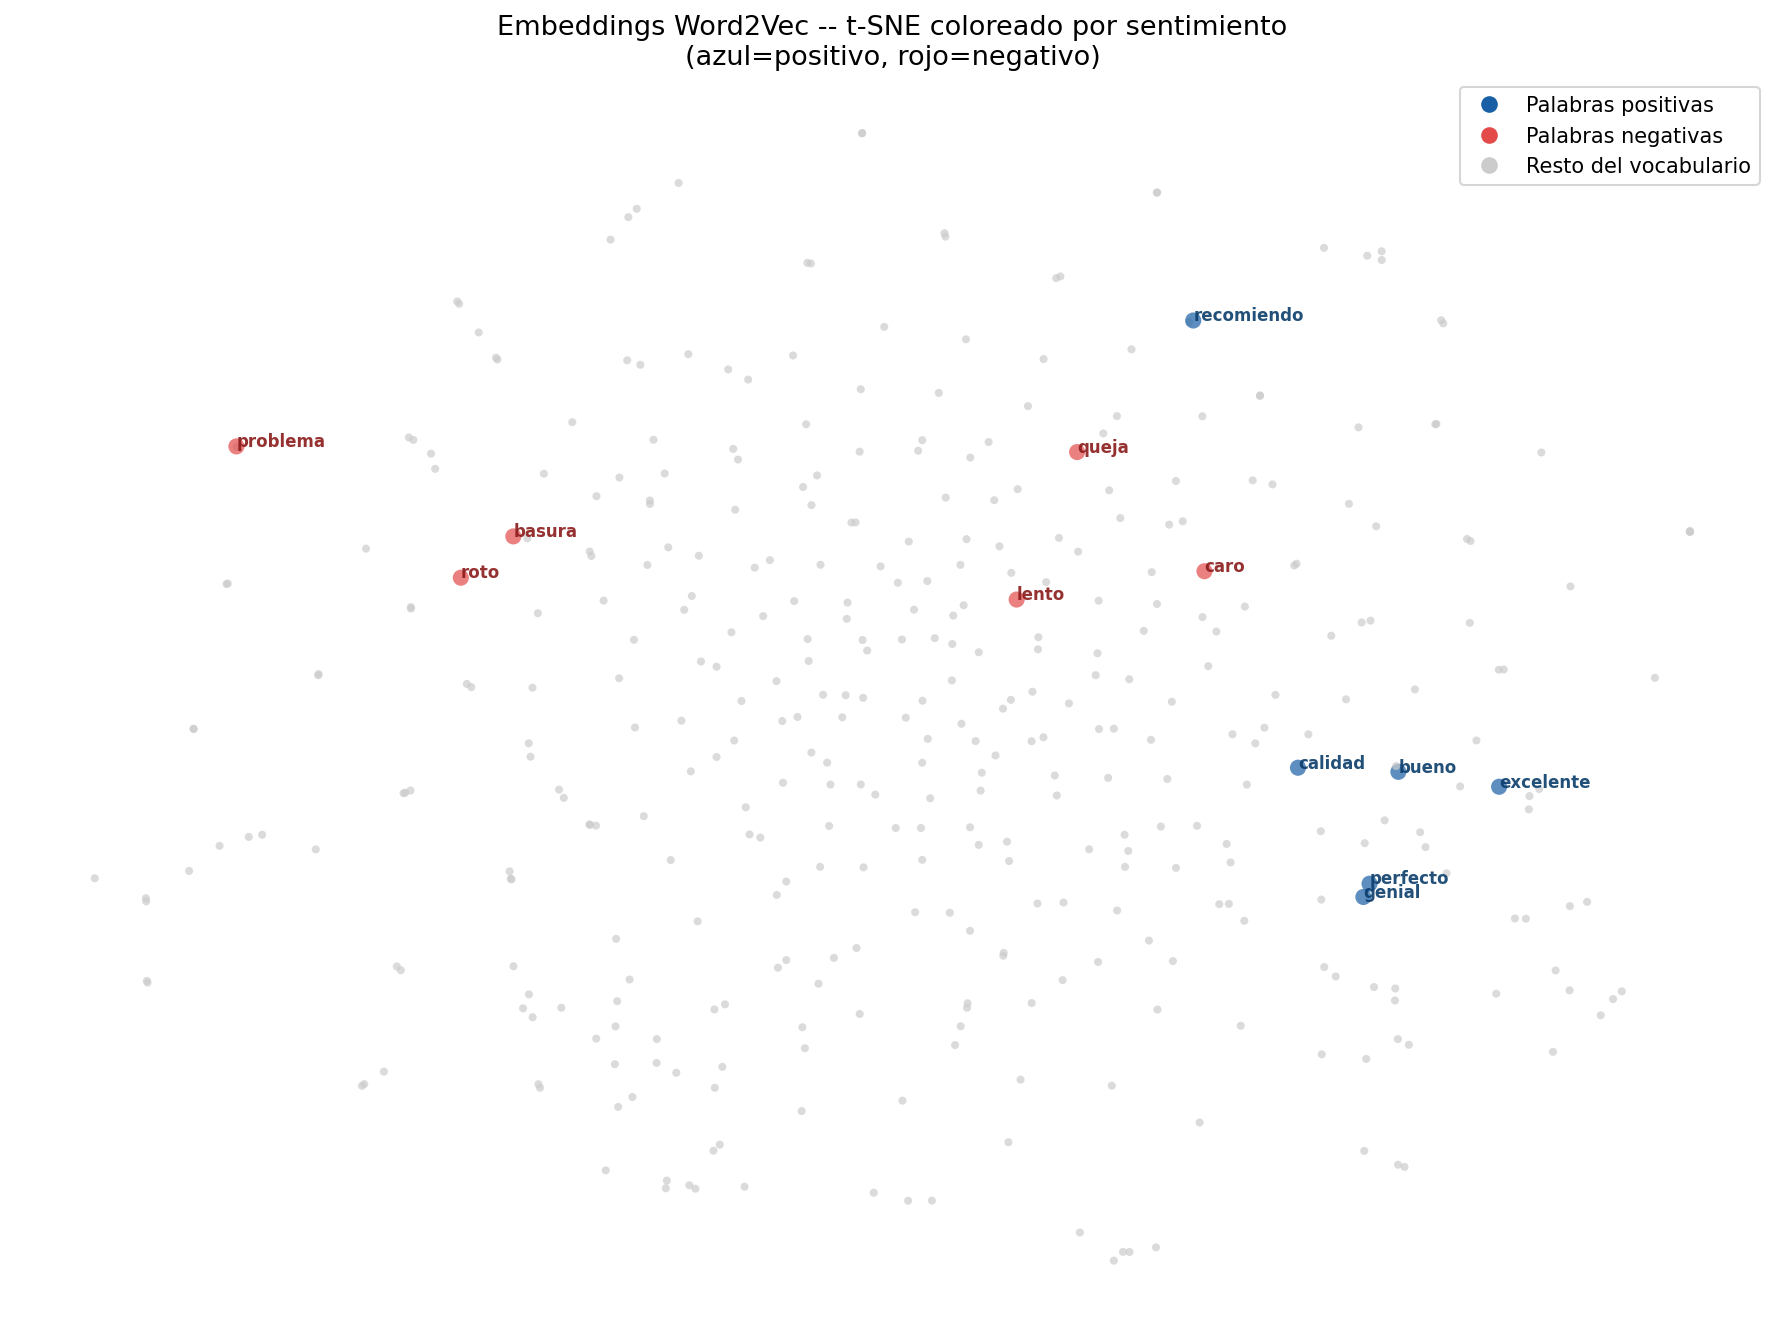
\includegraphics[width=0.68\textwidth]{exp4_tsne_colored.png}
\caption{t-SNE coloreado: azul = palabras positivas, rojo = negativas.}\label{fig:exp4}
\end{figure}

\subsection{Experimentos 5 y 5b: buscando los mejores ajustes}
¿Cuáles son la tasa y la dimensión ideales? Lo buscamos de dos formas: una rejilla ordenada
(probar combinaciones fijas) y una búsqueda Bayesiana con Optuna (que aprende de los intentos
anteriores para proponer mejores). Las dos llegan prácticamente al mismo lugar
(Cuadro~\ref{tab:exp5}). Importante: el óptimo de la rejilla quedó en el \emph{centro} del
rango probado (peor por encima y por debajo), señal de que buscamos en el lugar correcto.
\begin{figure}[H]
\centering
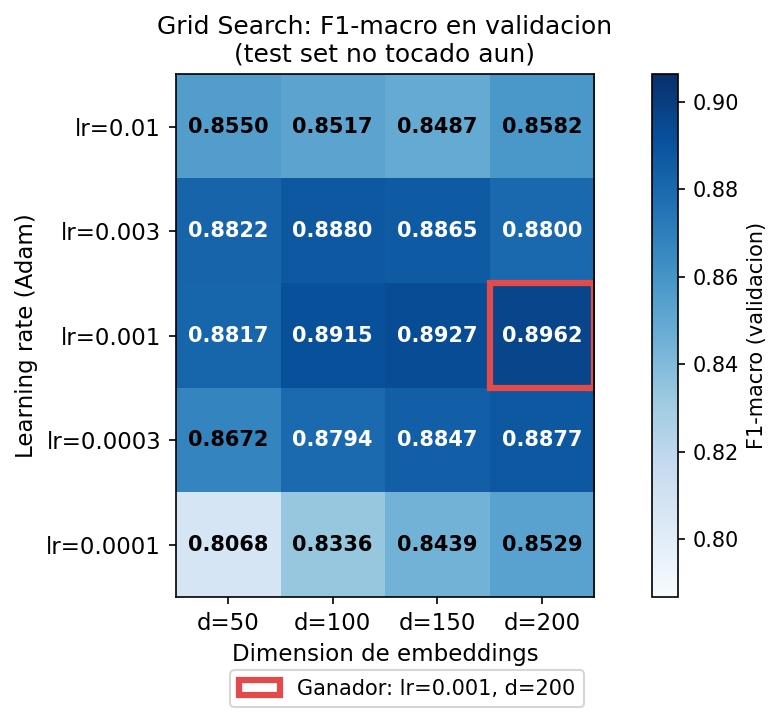
\includegraphics[width=0.58\textwidth]{exp5_grid_heatmap.png}
\caption{Mapa de calor de la rejilla. El óptimo ($\eta=0.001$, $d=200$) cae en el interior.}
\label{fig:exp5}
\end{figure}
\begin{table}[H]
\centering
\caption{Rejilla vs.\ búsqueda Bayesiana.}\label{tab:exp5}
\begin{tabular}{lccc}
\toprule
Método & Mejor config.\ & F1-val & F1-test \\
\midrule
Rejilla       & $\eta=0.001$, $d=200$    & 0.8962 & 0.8972 \\
Optuna (TPE)  & $\eta=0.00059$, $d=166$  & 0.8980 & 0.8970 \\
\bottomrule
\end{tabular}
\end{table}
\noindent\textbf{Qué significa.} La búsqueda Bayesiana, más sofisticada, no le ganó a la
rejilla. No siempre lo complejo paga: aquí el paisaje de validación es plano alrededor del
óptimo, así que una rejilla bien diseñada es más barata y igual de buena.

\subsection{Experimento 6: el duelo contra el gigante}\label{sec:exp6}
Este es el experimento que más nos hizo reflexionar. La pregunta era directa: nuestro
Word2Vec, entrenado con 40 mil reseñas, ¿puede competir con SBWC, unos embeddings
preentrenados con \textbf{1\,500 millones} de palabras? Para que la comparación fuera justa,
ambos usan el mismo clasificador y preprocesamiento; lo único que cambia es de dónde salen los
vectores. Medimos en tres escenarios: Amazon (nuestro dominio), y tuits en
español~\cite{barbieri2022} de dos formas ---transferencia (clasificador entrenado en Amazon y
probado en tuits) e ``in-domain'' (clasificador entrenado sobre los propios tuits)--- para
separar el efecto del cambio de tema del efecto de la calidad del vector.
\begin{table}[H]
\centering
\caption{El duelo (F1-macro). Mismo clasificador y preprocesamiento para todos.}
\label{tab:exp6}
\begin{tabular}{lccc}
\toprule
Representación & Amazon (su dominio) & Tuits (transfer.) & Tuits (in-domain) \\
\midrule
Nuestro W2V ($d=300$) & \textbf{0.9027} & 0.6733 & 0.7129 \\
SBWC preentrenado     & 0.8830 & \textbf{0.7529} & \textbf{0.7589} \\
TF-IDF (referencia)   & 0.9225 & 0.6829 & 0.7222 \\
\bottomrule
\end{tabular}
\end{table}
\noindent\textbf{Qué significa.} La respuesta intuitiva sería ``el gigante gana de calle'',
pero el resultado tiene un giro. En \emph{nuestro} dominio ---las reseñas de Amazon--- nuestro
modesto modelo le \emph{gana} al gigante ($0.903$ vs.\ $0.883$), porque conoce el vocabulario
específico: ``exelente'' mal escrito, ``no funciona'', nombres de productos. Pero al sacarlo de
su zona y evaluarlo con tuits ---un lenguaje informal, lleno de palabras que nunca vio--- la
situación se invierte y SBWC pasa al frente ($0.759$ vs.\ $0.713$). La explicación cabe en un
número: la \emph{cobertura} de vocabulario (Figura~\ref{fig:exp6}). De cada 100 palabras de
los tuits, nuestro modelo reconoce $82.7$ y SBWC, $96.4$. Las palabras que el modelo no
conoce simplemente desaparecen del promedio y, con ellas, parte de la señal. La variante
``in-domain'' confirma que la diferencia no es del clasificador sino del vector mismo: aun
entrenando sobre tuits, nuestro modelo choca con ese techo de vocabulario. La moraleja no es
``el preentrenado es mejor'', sino algo más fino: \textbf{lo especializado rinde mejor en su
dominio; lo general transfiere mejor fuera de él.}
\begin{figure}[H]
\centering
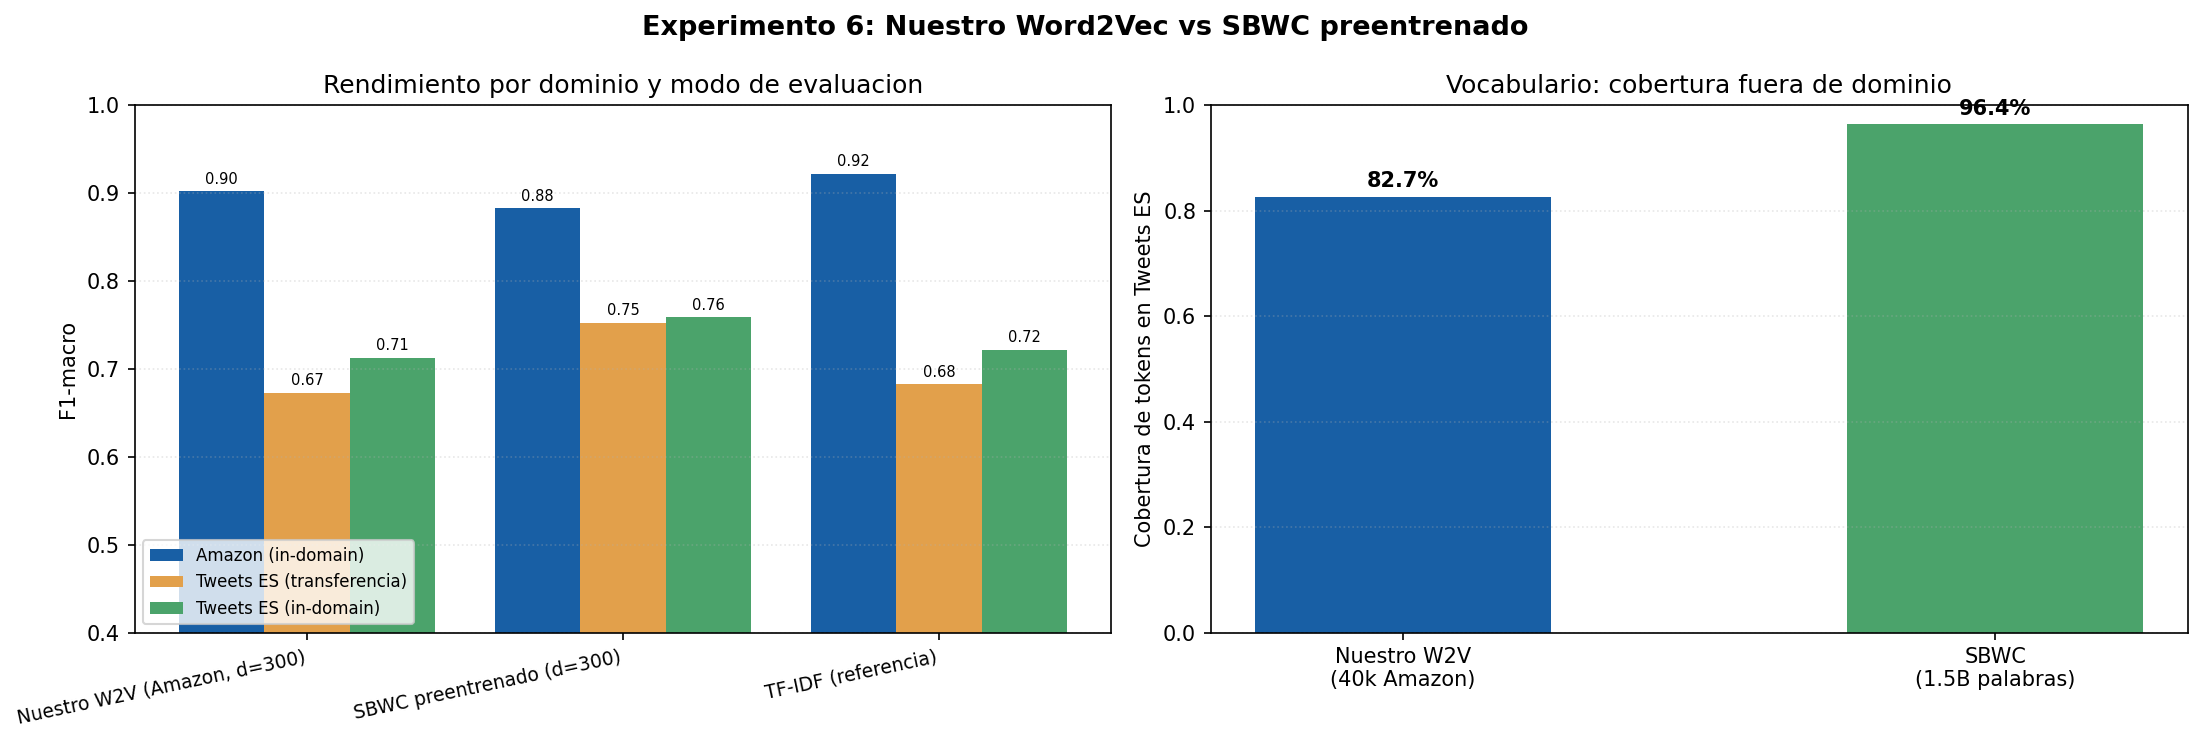
\includegraphics[width=\textwidth]{exp6_duelo_sbwc.png}
\caption{Duelo W2V vs.\ SBWC: rendimiento por dominio (izq.) y cobertura de vocabulario en los
tuits (der.).}\label{fig:exp6}
\end{figure}

\subsection{Verificación del gradiente}\label{sec:gradcheck}
Para cerrar el círculo entre la teoría y la práctica, comprobamos que el gradiente que
derivamos a mano (Ecuación~\eqref{eq:grad}) es realmente correcto. Lo comparamos contra dos
referencias: (A) la diferenciación automática de PyTorch y (B) un gradiente numérico calculado
por diferencias finitas (mover un poquito cada parámetro y ver cuánto cambia la pérdida). Las
tres coinciden: el error máximo entre nuestra fórmula y la automática es del orden de
$10^{-16}$, y la prueba de diferencias finitas pasa. En otras palabras, no solo escribimos la
fórmula bonita: comprobamos que el modelo minimiza la pérdida exacta con su gradiente exacto.

% ============================================================
\section{Análisis y discusión}\label{sec:analisis}
Volvamos a las hipótesis y veamos cuáles aguantaron.

\paragraph{H1 (confirmada, con matiz).} A igual tasa ($\eta=0.001$), los adaptativos le sacan
mucha ventaja a SGD, que se queda atascado (exp2). Pero ojo: eso no significa que SGD sea peor.
Con su propia tasa ($\eta=0.1$) llega a $0.861$, a solo $\sim$3 puntos del mejor. La diferencia
es de \emph{ajuste}, no de talento del algoritmo.

\paragraph{H3 (confirmada).} SGD es muy sensible a la tasa: barre de $0.62$ a $0.87$ según el
paso (exp1), mientras Adam funciona bien en un rango amplio. El exp2 explica el mecanismo: la
inicialización en ceros crea una meseta casi plana, y solo la inercia y la adaptación del paso
permiten escapar de ella.

\paragraph{H2 (refutada, con matiz).} La segunda capa no mejoró la clasificación: el mejor
modelo sigue siendo 1 capa con RMSProp ($0.8940$). Curiosamente, esa capa extra \emph{sí}
ayuda al optimizador más débil (SGD sube de $0.861$ a $0.881$): la no linealidad cambia el
terreno de una forma que le conviene a SGD, aunque no mueva la aguja del mejor modelo global.

\paragraph{H4 (refutada).} El resultado más instructivo del trabajo. TF-IDF nos gana, y lo
hace incluso con palabras sueltas ($0.9107$ vs.\ $0.8990$), así que no es cuestión de pares de
palabras. Refleja una propiedad del dominio: en reseñas de productos, las palabras clave por sí
solas bastan. No es una derrota de Word2Vec, es honestidad sobre cuándo conviene cada
herramienta.

\paragraph{H5 (refutada).} La búsqueda Bayesiana no superó significativamente a la rejilla
($0.8970$ vs.\ $0.8972$). El óptimo es interior y el paisaje, plano: una rejilla bien pensada
fue más costo-efectiva.

\paragraph{H6 (confirmada, con el matiz más interesante).} SBWC generaliza mejor fuera de
dominio ($0.759$ vs.\ $0.713$ en tuits), respaldado por la cobertura ($96.4\%$ vs.\ $82.7\%$).
Pero dentro de dominio la cosa se invierte: nuestro modelo le gana en Amazon ($0.903$ vs.\
$0.883$). No hay un ganador absoluto, hay un \emph{trade-off de dominio}.

\paragraph{Interpretabilidad.} El exp4 confirma que los vectores tienen significado real
(excelente $\to$ inmejorable, roto $\to$ doblado). Poder ``leer'' lo que aprendió el modelo es
una ventaja frente a métodos más opacos.

\paragraph{Sobre nuestras decisiones de diseño.} Para que no parezcan azar: (i) cada
optimizador usó su tasa adecuada, porque compararlos con la misma sería injusto; (ii) exp1 y
exp2 usan 7 épocas en vez de 5 para darle tiempo a la dinámica lenta de SGD; (iii) los
experimentos de afinación usan Adam, que está empatado con RMSProp ($<0.001$) y es el estándar;
(iv) el duelo usa $d=300$ para igualar la dimensión de SBWC, dentro de la meseta de rendimiento.

% ============================================================
\section{Fortalezas, limitaciones y usos profesionales}

\subsection{Fortalezas}
\textbf{Eficiencia:} nuestro Word2Vec representa cada reseña con 300 números y queda a 1--2
puntos de un TF-IDF de 50\,000 características. Quedar tan cerca usando 167 veces menos números
es, en realidad, una virtud. \textbf{Transferibilidad:} los vectores se reutilizan en otras
tareas, como mostró el duelo fuera de dominio. \textbf{Interpretabilidad:} distancia entre
vectores $=$ similitud de significado (exp4). \textbf{Sin etiquetas:} se entrena solo con
texto crudo.

\subsection{Limitaciones}
\textbf{Vectores estáticos:} ``banco'' (de plata) y ``banco'' (de sentarse) comparten un único
vector. \textbf{Vocabulario cerrado:} las palabras nuevas no tienen representación ---lo
medimos en el exp6, donde nuestra cobertura fuera de dominio fue del $82.7\%$ frente al
$96.4\%$ de SBWC. \textbf{Promedio del documento:} al promediar se pierde el orden de las
palabras, y con él los matices que dependen de la estructura de la frase.

\subsection{Usos actuales en el ámbito profesional}
Word2Vec y sus variantes siguen muy vivos: en motores de recomendación (tratando productos
como ``palabras'' en secuencias de compra), en búsqueda semántica y recuperación de
información, en análisis de sentimiento y enrutamiento de tickets de atención al cliente,
en expansión de consultas, y como punto de partida para modelos más grandes. Su bajo costo,
su velocidad y su interpretabilidad lo mantienen como una herramienta de primera línea cuando
importan la latencia y los recursos.

% ============================================================
\section{Conclusiones}\label{sec:conclusiones}
\begin{enumerate}
  \item \textbf{H1 confirmada:} a igual tasa, Adam y RMSProp convergen y SGD se atasca
  (gradiente $\sim$80$\times$ menor); pero con su tasa, SGD llega a $0.861$. El factor decisivo
  es el ajuste, no el algoritmo.
  \item \textbf{H2 refutada:} la segunda capa no mejora la clasificación. El mejor modelo es
  1 capa con RMSProp (F1$=0.8940$).
  \item \textbf{H3 confirmada:} SGD exige ajuste fino de la tasa (F1 de $0.62$ a $0.87$); Adam
  es robusto.
  \item \textbf{H4 refutada:} TF-IDF supera a Word2Vec incluso con palabras sueltas ($0.9107$
  vs.\ $0.8990$); el vocabulario directo de las reseñas favorece al método clásico.
  \item \textbf{H5 refutada:} la búsqueda Bayesiana no mejora a la rejilla; el óptimo es
  interior y el paisaje, plano.
  \item \textbf{H6 confirmada con matiz:} SBWC generaliza mejor fuera de dominio, pero nuestro
  modelo lo supera en su propio dominio. Es un trade-off, no un ganador absoluto.
  \item \textbf{Para el curso:} Word2Vec resultó un caso de estudio ideal de optimización ---
  pudimos ver la función de pérdida, derivar y \emph{verificar} su gradiente, comparar
  algoritmos de minimización y buscar hiperparámetros--- todo sobre un problema real de NLP en
  español.
\end{enumerate}

% ============================================================
\begin{thebibliography}{9}
\bibitem{harris1954} Z. S. Harris. \emph{Distributional structure}. Word, 10(2--3):146--162, 1954.
\bibitem{keung2020} P. Keung, Y. Lu, G. Szarvas, N. A. Smith. \emph{The Multilingual Amazon Reviews Corpus}. EMNLP, 2020.
\bibitem{kingma2014} D. P. Kingma, J. Ba. \emph{Adam: A Method for Stochastic Optimization}. arXiv:1412.6980, 2014.
\bibitem{mikolov2013a} T. Mikolov, K. Chen, G. Corrado, J. Dean. \emph{Efficient Estimation of Word Representations in Vector Space}. arXiv:1301.3781, 2013.
\bibitem{mikolov2013b} T. Mikolov, I. Sutskever, K. Chen, G. Corrado, J. Dean. \emph{Distributed Representations of Words and Phrases and their Compositionality}. NeurIPS, 2013.
\bibitem{muennighoff2023} N. Muennighoff, N. Tazi, L. Magne, N. Reimers. \emph{MTEB: Massive Text Embedding Benchmark}. arXiv:2210.07316, 2023.
\bibitem{barbieri2022} F. Barbieri, L. Espinosa Anke, J. Camacho-Collados. \emph{XLM-T: Multilingual Language Models in Twitter for Sentiment Analysis and Beyond}. LREC, 2022.
\end{thebibliography}

\end{document}
